\documentclass[11pt,a4paper]{article}
\usepackage[utf8]{inputenc}
\usepackage[T1]{fontenc}
\usepackage[spanish,es-nodecimaldot]{babel}
\usepackage{geometry}
\usepackage{amsmath,amssymb}
\usepackage{booktabs}
\usepackage{graphicx}
\usepackage{listings}
\usepackage{xcolor}
\usepackage{siunitx}
\usepackage{hyperref}
\usepackage{float}
\usepackage{microtype}
\usepackage{csquotes}
\usepackage[backend=biber,style=ieee]{biblatex}

\addbibresource{references_U4.bib}
\geometry{margin=2.5cm}
\sisetup{output-decimal-marker={,}}
\graphicspath{{../salida_pe_u4/figs/}{../evidencia/}}
\hypersetup{colorlinks=true,linkcolor=blue,citecolor=blue,urlcolor=blue}
\emergencystretch=2em
\lstset{basicstyle=\ttfamily\small,breaklines=true,frame=single,numbers=left,
  keywordstyle=\color{blue},commentstyle=\color{green!40!black},
  stringstyle=\color{orange!60!black}}

% Este documento contiene únicamente el aporte redactado por José Alejandro
% Lozano Morales. Los bloques pendientes deben ser completados personalmente
% por Andy Sánchez e Isaías Urbina, con sus propias fuentes y redacción.
\newcommand{\pendiente}[2]{%
  \begin{center}
  \fbox{\parbox{0.92\textwidth}{\textbf{Pendiente de #1.} #2}}
  \end{center}}

\title{\textbf{GA-SUM-05 / PE-U4}\\Procesamiento distribuido con Apache Spark:\\comprobación experimental de la Ley de Amdahl aplicada a FUVV}
\author{José Alejandro Lozano Morales\\Andy Paul Sánchez Pilaloa\\Isaías Abraham Urbina Romero}
\date{Período académico 2026--2027 PPA}

\begin{document}
\maketitle
\begin{center}
Universidad Técnica Estatal de Quevedo\\
Facultad de Ciencias de la Computación\\
Carrera de Ingeniería de Software\\
Aplicaciones Distribuidas (ISR-701)\\[1em]
PFC de referencia: \textbf{FUVV -- Laboratorios Informáticos}
\end{center}

\noindent\textbf{Integrantes, PFC de origen y roles.}
José Alejandro Lozano Morales (AGLS -- TiendaTech), coordinador de experimentación y reproducibilidad;
Andy Paul Sánchez Pilaloa (AGLS -- TiendaTech), responsable de datos y documentación científica;
Isaías Abraham Urbina Romero (FUVV -- Laboratorios Informáticos), responsable de PySpark y verificación.

\section*{Justificación del PFC de referencia}
El sistema FUVV administra solicitudes, reservas, horarios y utilización de infraestructura en múltiples laboratorios. La acumulación histórica de eventos por usuario, asignatura, laboratorio y franja horaria permite plantear operaciones de filtrado, agregación, unión y priorización que crecen con cada período académico. El pipeline desarrollado apoya decisiones sobre redistribución de horarios, identificación de saturación recurrente y ampliación de capacidad. Al no disponerse de una base institucional anonimizada y con licencia pública, se empleó un conjunto sintético declarado, construido a partir del esquema del PFC, con semilla fija y sin datos personales reales. Esta decisión permite conservar las relaciones entre solicitudes, laboratorios, perfiles y materias, a la vez que garantiza que cualquier integrante pueda reproducir el experimento desde el código publicado.

\newpage
\tableofcontents
\newpage

\begin{abstract}
Se comparó un pipeline secuencial implementado con pandas y su equivalente con PySpark sobre 520,000 solicitudes sintéticas del dominio FUVV. Cinco transformaciones independientes se midieron con una ejecución de calentamiento descartada y cinco repeticiones cronometradas; la mediana se utilizó como estadístico principal. En la configuración base, pandas fue más rápido en las cinco operaciones: el speedup frente a Spark varió entre 0,1282 para T1 y 0,8064 para T5. Para T3, el tiempo de Spark descendió de \SI{11.980450}{\second} con una unidad local a \SI{9.909173}{\second} con cuatro, con un speedup interno de 1,2090 y eficiencia de 0,3023. Los resultados muestran que, para este volumen y una máquina virtual con recursos limitados, la sobrecarga de planificación, serialización y shuffle domina el beneficio del paralelismo. El trabajo conserva código, mediciones, figuras y evidencia de Spark UI para facilitar su reproducción.
\end{abstract}

\section{Introducción}
El procesamiento paralelo distribuye trabajo entre varias unidades de ejecución, pero el aumento de recursos no garantiza una reducción proporcional del tiempo. Una parte de la aplicación permanece secuencial y el motor introduce actividades adicionales, como planificación, comunicación, serialización y redistribución de datos. Por eso, la evaluación de rendimiento debe apoyarse en mediciones y no en la suposición de que una plataforma distribuida siempre supera a una biblioteca local.

La práctica implementa cinco transformaciones equivalentes en pandas y PySpark sobre datos del dominio FUVV. El objetivo es calcular el speedup experimental, estudiar el escalamiento de T3 con una, dos y cuatro unidades locales y contrastar el resultado con la Ley de Amdahl. La literatura reciente insiste en que las leyes de Amdahl y Gustafson--Barsis describen perspectivas relacionadas del escalamiento, siempre que se distingan la carga fija y la carga creciente \cite{karbowski2025}. Asimismo, el rendimiento de Spark depende del volumen, la configuración y la complejidad de la aplicación, por lo que una predicción útil debe considerar simultáneamente esas variables \cite{shen2023spark}.

\section{Fundamento teórico}
\subsection{Paralelismo y leyes de escalamiento}
El paralelismo de datos aplica una operación equivalente a particiones diferentes de una colección, mientras el paralelismo de tareas permite que actividades distintas progresen de manera concurrente. En ambos casos existen dependencias que impiden dividir todo el trabajo. La Ley de Amdahl representa una carga fija mediante una fracción paralelizable $p$ y una fracción secuencial $1-p$. Si el tiempo con una unidad se normaliza a uno, la parte paralela consume $p/N$ al utilizar $N$ unidades, por lo que
\begin{equation}
S(N)=\frac{1}{(1-p)+\frac{p}{N}}.
\label{eq:amdahl}
\end{equation}
Cuando $N$ tiende a infinito, la parte paralela se aproxima a cero, pero la parte secuencial permanece:
\begin{equation}
S_{\max}=\lim_{N\to\infty}S(N)=\frac{1}{1-p}.
\label{eq:smax}
\end{equation}

Karbowski demuestra que las formulaciones de Amdahl y Gustafson--Barsis pueden transformarse directamente una en otra al unificar la definición de la fracción secuencial y reconocer como constante el tiempo de esa parte para un problema dado \cite{karbowski2025}. La diferencia principal no consiste en leyes incompatibles, sino en la perspectiva de escalamiento. Amdahl mantiene fijo el tamaño del problema; Gustafson--Barsis considera que el trabajo paralelizable puede aumentar con los recursos:
\begin{equation}
S_G(N)=N-(1-p)(N-1).
\label{eq:gustafson}
\end{equation}
La eficiencia expresa cuánto speedup se obtiene por unidad utilizada:
\begin{equation}
E(N)=\frac{S(N)}{N}.
\label{eq:eficiencia}
\end{equation}
Estas expresiones son límites ideales porque omiten comunicación, sincronización y creación de tareas. En un motor real, los valores medidos pueden quedar por debajo de la curva e incluso producir speedup menor que uno.

\subsection{MapReduce, Hadoop y heterogeneidad}
MapReduce divide una carga en funciones de mapeo y reducción. Los mappers transforman registros de entrada en pares intermedios; luego el sistema particiona, transfiere y ordena los pares por clave mediante el shuffle; finalmente, los reducers combinan los valores y escriben la salida. Hadoop incorpora HDFS para almacenamiento distribuido y YARN para administrar recursos y ejecuciones. Esta separación facilita trabajar con grandes colecciones, pero las escrituras intermedias y el movimiento de datos generan una sobrecarga apreciable.

La heterogeneidad del hardware vuelve especialmente importante la planificación. Lim y Park estudiaron clústeres Hadoop compuestos por computadoras de placa única con capacidades diferentes y observaron que la asignación uniforme puede sobrecargar los nodos débiles y aumentar la variación entre ejecuciones \cite{lim2024hadoop}. Su propuesta modifica políticas de YARN para considerar los recursos reales de cada nodo y reporta mejoras medias de 2,55 veces en cargas intensivas de entrada/salida y 1,55 veces en cargas intensivas de CPU. Este resultado no significa que toda carga Hadoop alcance esas ganancias; demuestra que la arquitectura, el tipo de operación y la distribución de recursos condicionan el rendimiento.

En la práctica FUVV se emplea una máquina virtual local, no un clúster Hadoop. Sin embargo, la lección es aplicable: declarar cuatro hilos no equivale a disponer de cuatro núcleos físicos independientes. La máquina de Colab reportó dos núcleos, por lo que la configuración \texttt{local[4]} introduce sobresuscripción. Esa limitación debe incorporarse al análisis, pues explica parte de la eficiencia decreciente observada.

\subsection{Rendimiento de Apache Spark}
Spark representa las operaciones mediante un grafo acíclico dirigido y las organiza en jobs, stages y tasks. Las transformaciones son perezosas: construyen un plan que solo se ejecuta cuando una acción materializa el resultado. En este experimento la materialización se fuerza mediante una escritura al destino \texttt{noop}; así se evita medir únicamente la construcción del plan. Las operaciones con dependencias amplias, como agrupaciones y joins, requieren \emph{shuffle}, lo que añade serialización, transferencia y espera entre etapas.

El tiempo de una aplicación Spark depende del tamaño de la entrada, la capacidad de cómputo, la configuración y la complejidad del algoritmo. Shen, Chen y Rao señalan que la predicción de rendimiento debe representar conjuntamente esas variables y proponen un modelo multitarea para estimar tiempos de varias aplicaciones Spark \cite{shen2023spark}. Esta observación respalda una lectura prudente de la práctica: un único speedup no constituye una propiedad universal de Spark, sino el resultado de una combinación concreta de datos, transformación y entorno.

La captura de Spark UI de T3 muestra un job completado con siete stages, ocho tareas por stage y varios intercambios. El DAG confirma que la unión de cuatro DataFrames no es una operación local sencilla; contiene redistribuciones antes de producir la salida. Por ello, aun cuando cuatro hilos reducen el tiempo respecto de una unidad, el coste fijo y el shuffle impiden superar a pandas con 520,000 registros.

\subsection{Computación en la nube y modelo serverless}
La nube permite aprovisionar capacidad sin administrar necesariamente el hardware físico. En IaaS el usuario conserva mayor control sobre máquinas y redes; PaaS abstrae el entorno de ejecución; SaaS entrega una aplicación terminada; y FaaS ejecuta funciones activadas por eventos. El modelo serverless traslada al proveedor tareas de aprovisionamiento y escalamiento, y cobra con una granularidad asociada al consumo. Sin embargo, no elimina los costes técnicos: arranques en frío, gestión de estado, comunicación entre funciones y dependencia del proveedor pueden afectar el rendimiento.

La revisión sistemática de Wen y colaboradores analizó 164 trabajos y organizó 17 direcciones de investigación sobre serverless, entre ellas optimización de rendimiento, marcos de programación, migración, desarrollo multinube, pruebas y depuración \cite{wen2023serverless}. Esto muestra que FaaS no constituye una sustitución automática de Spark. Las funciones son apropiadas para eventos breves y desacoplados; un pipeline analítico con joins amplios, estado y grandes transferencias puede requerir un motor especializado o un servicio administrado de Spark.

Para FUVV podría utilizarse FaaS para validar una solicitud nueva, publicar un evento o activar un flujo, mientras Spark procesaría lotes históricos de reservas. Esta separación evita mantener un clúster activo para operaciones pequeñas y reserva el motor distribuido para cargas que justifiquen su sobrecarga. La decisión debe considerar periodicidad, volumen, latencia y coste, no únicamente la disponibilidad de una tecnología.

\pendiente{Andy e Isaías}{Añadir sus aportes teóricos personales y sus referencias. Cada afirmación nueva debe citar una fuente que ellos hayan verificado. El informe final requiere al menos ocho referencias, seis con DOI o ISBN.}

\section{Materiales y método}
El experimento se ejecutó en Google Colab con Python 3.12.13, PySpark 3.5.0, pandas 2.2.2 y NumPy 2.0.2. La máquina virtual reportó dos núcleos. El generador produjo 520,000 solicitudes, 286,216 reservas, 15,000 perfiles, 120 laboratorios y 12 materias mediante la semilla 20260808. Cada transformación se ejecutó de forma independiente. Se descartó una ejecución de calentamiento y se midieron cinco repeticiones con \texttt{time.perf\_counter()}; se reportó la mediana y el coeficiente de variación.

Las transformaciones fueron: T1, filtrado compuesto; T2, agrupación con cinco agregaciones; T3, unión de cuatro DataFrames por UUID; T4, columnas derivadas de duración, franja y demanda; y T5, ordenamiento con selección de los 100 primeros registros. En PySpark se fijaron ocho particiones para que el algoritmo no cambiara al variar la concurrencia. T3 se midió con \texttt{local[1]}, \texttt{local[2]} y \texttt{local[4]}. La equivalencia entre motores se verificó mediante cardinalidad, número de columnas y firmas agregadas; las cinco transformaciones resultaron equivalentes.

\pendiente{Andy}{Insertar los fragmentos de código pandas solicitados por la guía mediante \texttt{lstlisting}, con \texttt{caption} y \texttt{label}.}
\pendiente{Isaías}{Insertar los fragmentos PySpark y describir la configuración efectiva de Spark obtenida durante la corrida.}

\section{Resultados}
\begin{table}[H]
\centering
\caption{Tiempos medianos y speedup de pandas frente a PySpark.}
\label{tab:tiempos}
\begin{tabular}{lSSS}
\toprule
{Transformación} & {$T_{pandas}$ (s)} & {$T_{Spark}$ (s)} & {$S=T_{pandas}/T_{Spark}$} \\
\midrule
T1 & 0.102893 & 0.802504 & 0.1282 \\
T2 & 0.130419 & 0.753264 & 0.1731 \\
T3 & 1.510329 & 11.277967 & 0.1339 \\
T4 & 0.323776 & 0.934518 & 0.3465 \\
T5 & 0.415923 & 0.515745 & 0.8064 \\
\bottomrule
\end{tabular}
\end{table}

\begin{figure}[H]
\centering
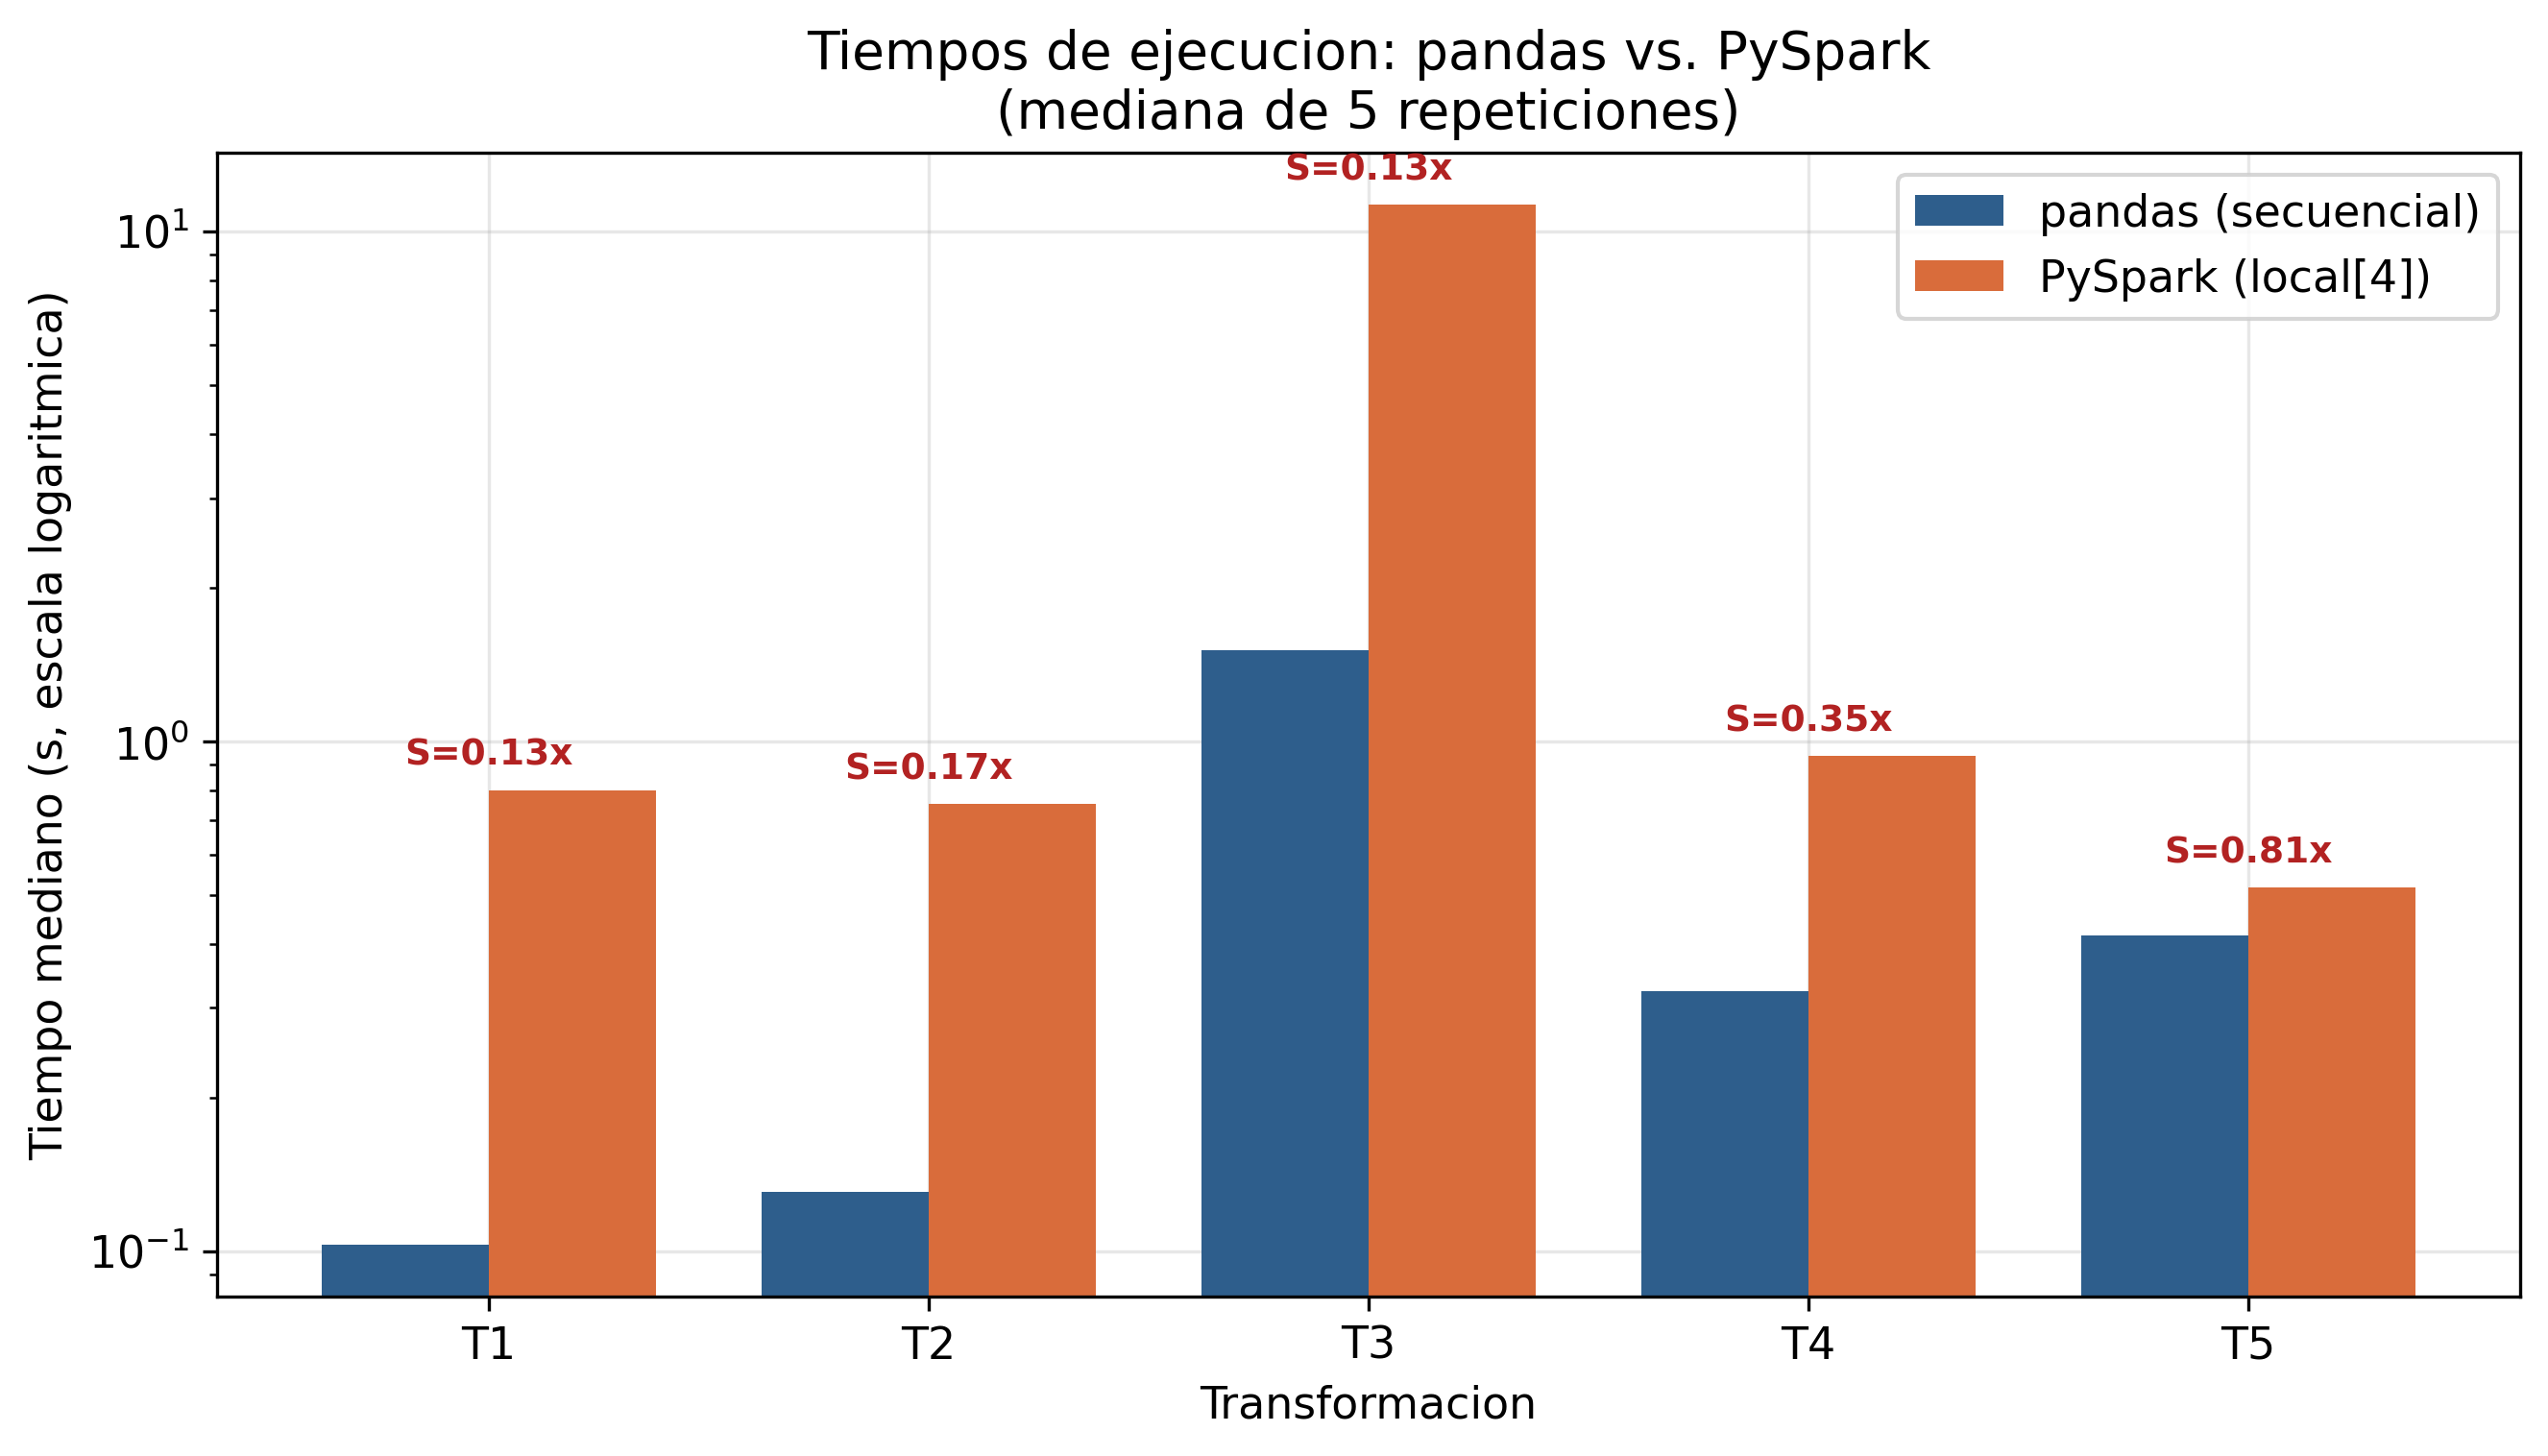
\includegraphics[width=.9\textwidth]{fig_a_tiempos.png}
\caption{Comparación de tiempos medianos entre pandas y PySpark.}
\label{fig:tiempos}
\end{figure}
La figura~\ref{fig:tiempos} confirma que Spark fue más lento en las cinco operaciones. La brecha mayor aparece en T3: la mediana pasa de \SI{1.510329}{\second} en pandas a \SI{11.277967}{\second} en Spark. T5 es el caso más cercano al equilibrio, con speedup 0,8064. El resultado es coherente con un volumen moderado, costes fijos de la JVM y una máquina virtual con dos núcleos.

\begin{figure}[H]
\centering
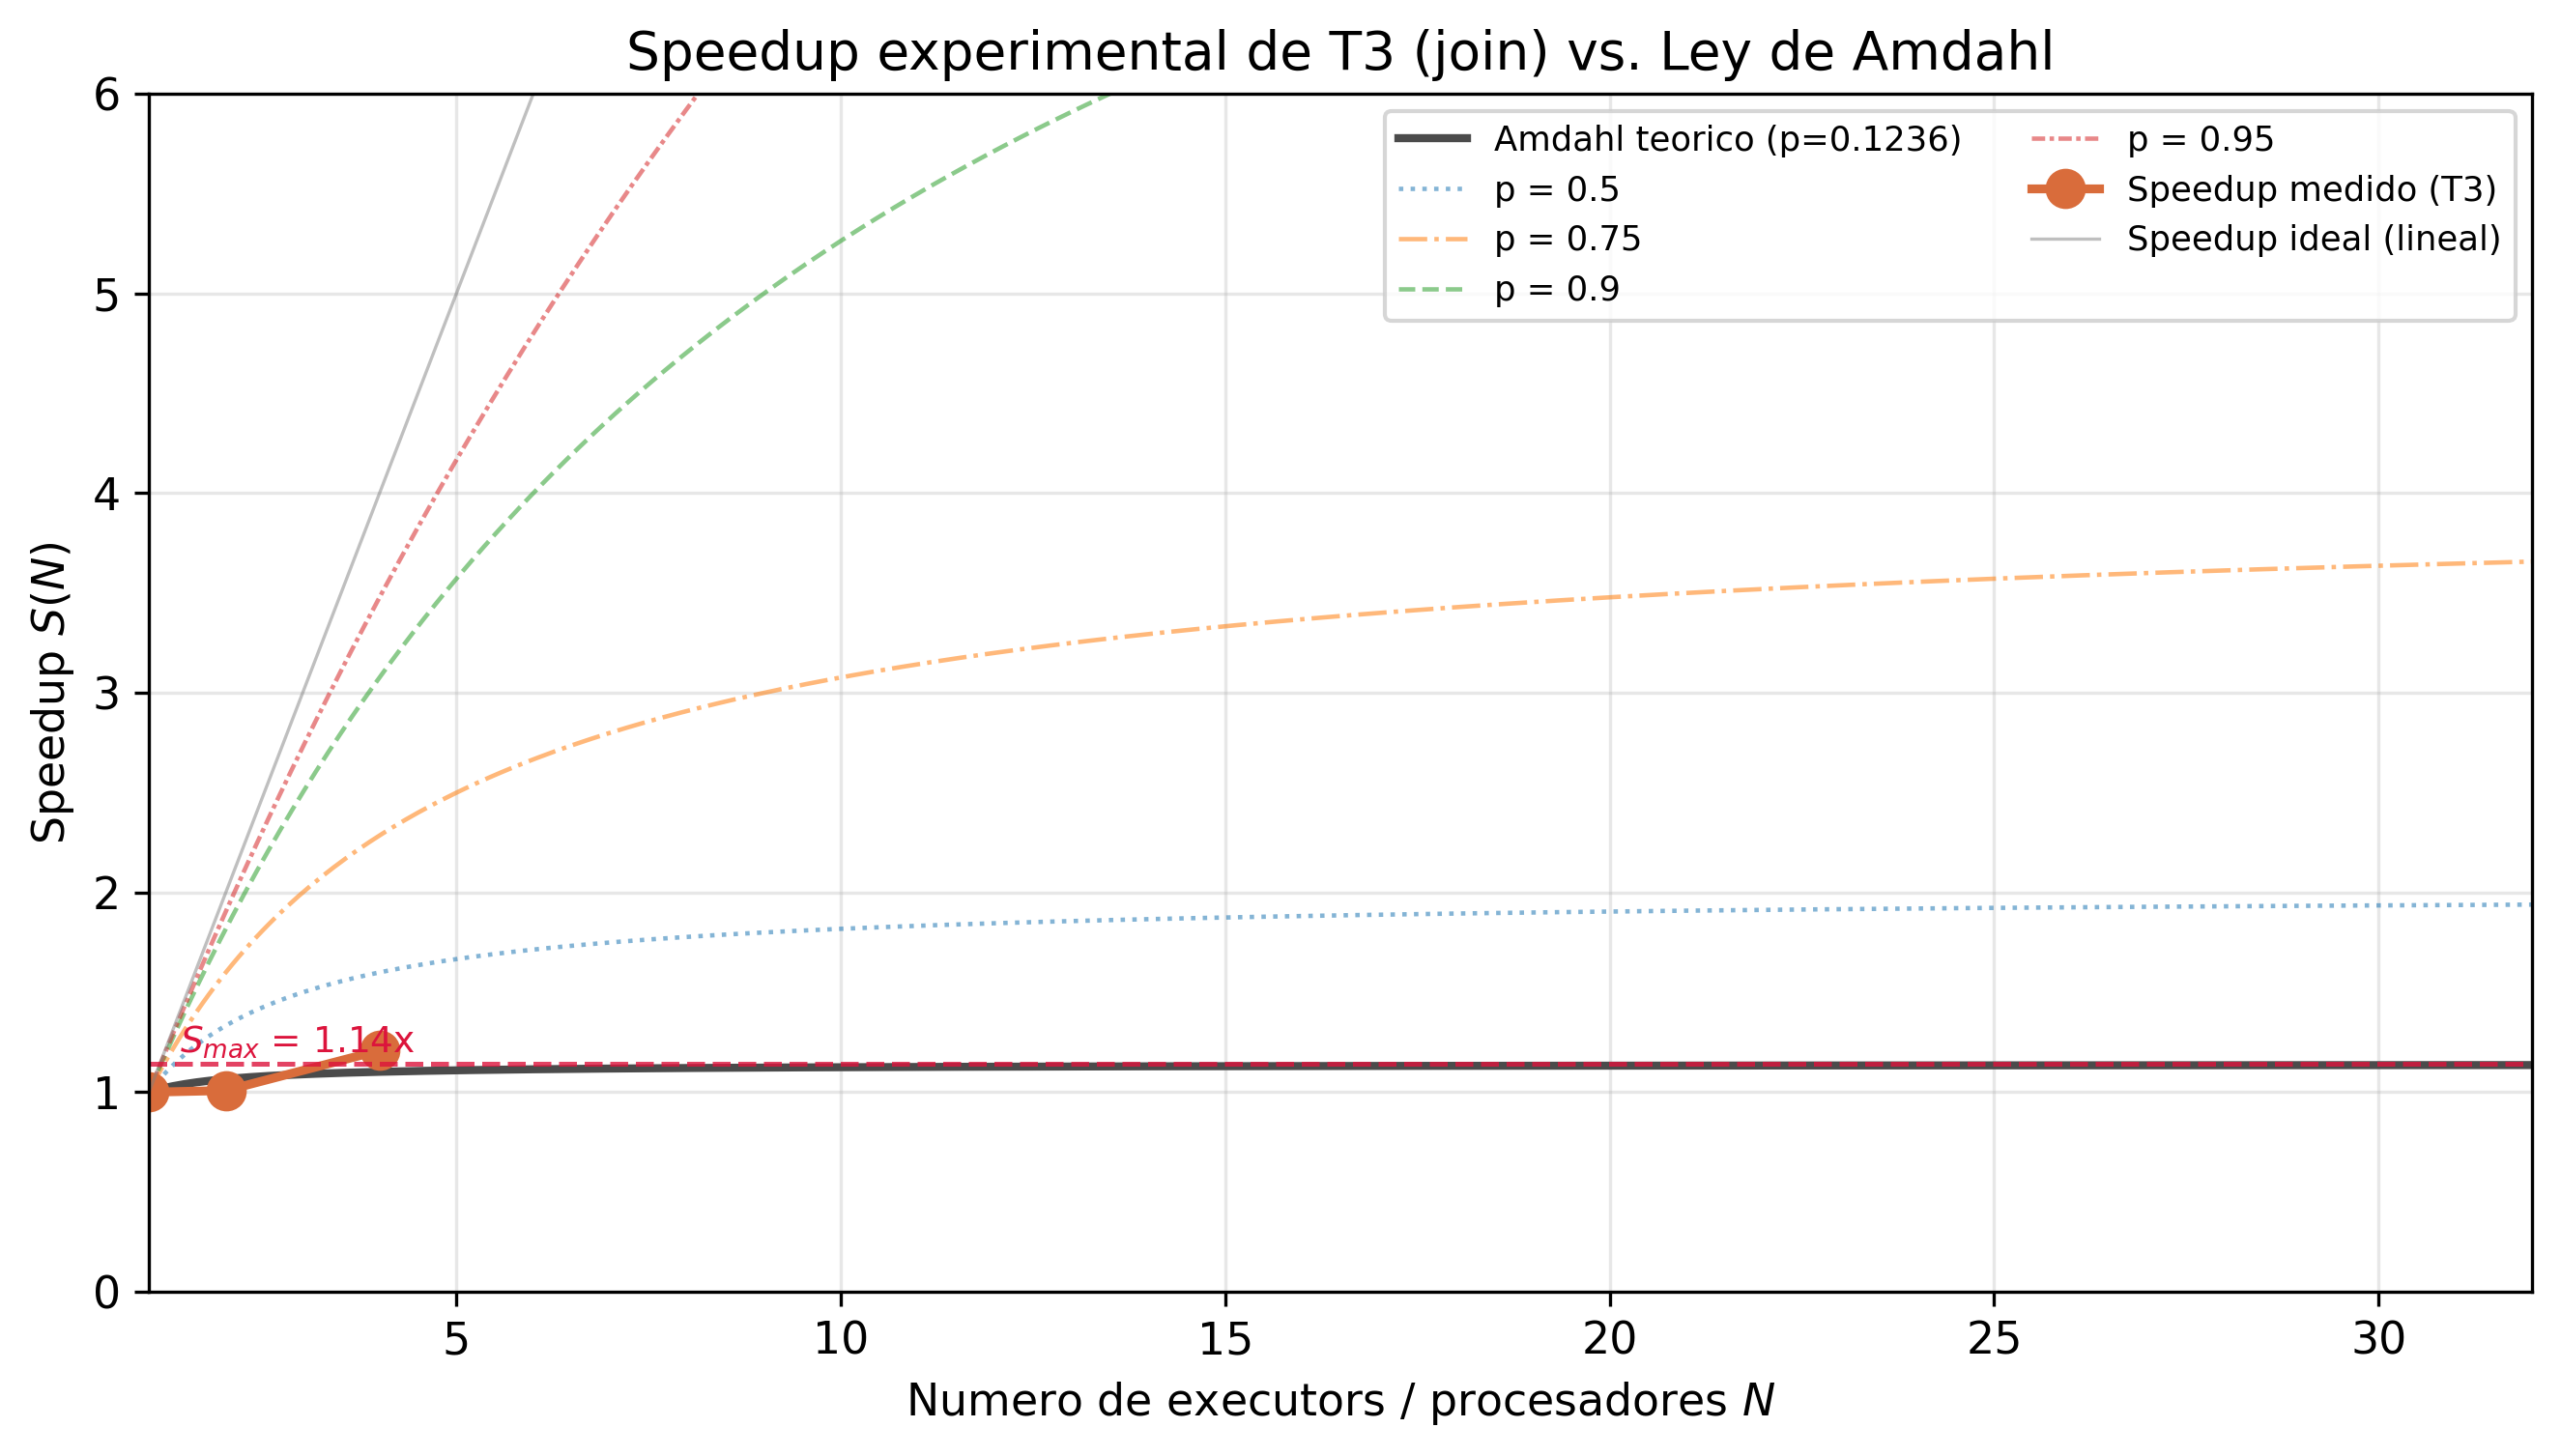
\includegraphics[width=.9\textwidth]{fig_b_speedup_amdahl.png}
\caption{Speedup interno de T3 y curva de Amdahl.}
\label{fig:speedup}
\end{figure}

\begin{figure}[H]
\centering
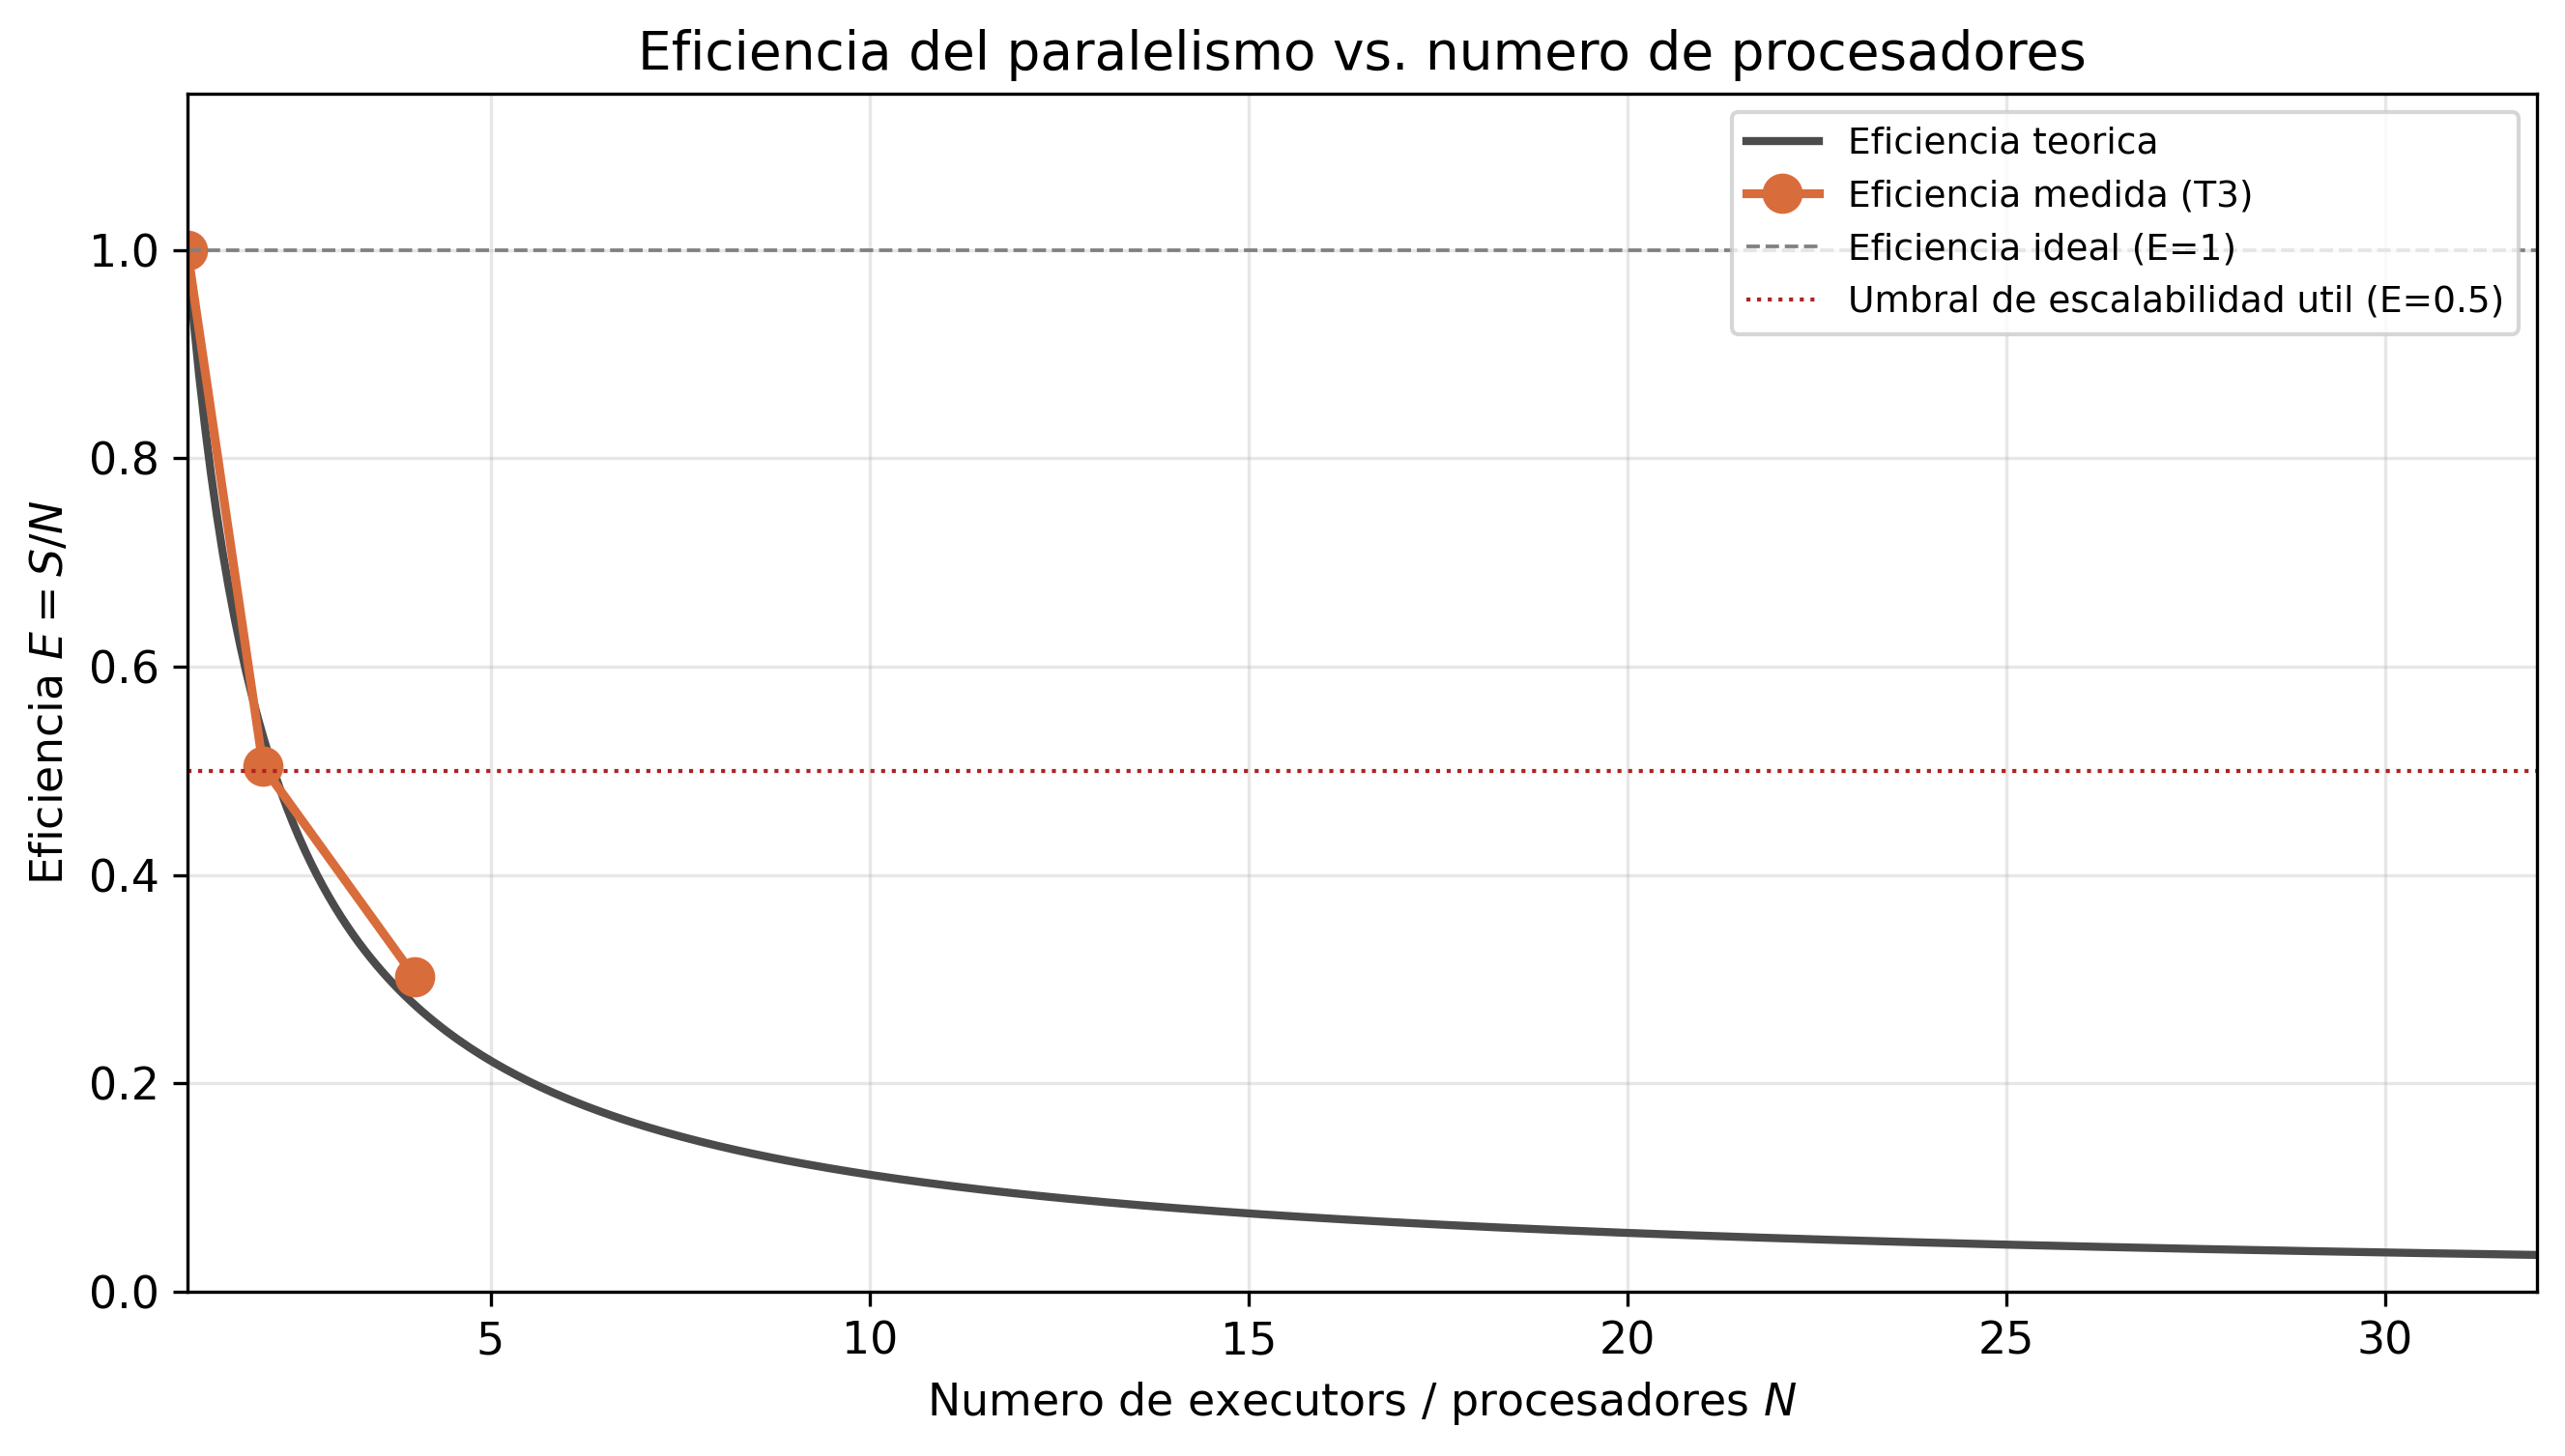
\includegraphics[width=.9\textwidth]{fig_c_eficiencia.png}
\caption{Eficiencia observada durante el escalamiento de T3.}
\label{fig:eficiencia}
\end{figure}
El speedup interno de T3 pasa de 1,0000 con $N=1$ a 1,0084 con $N=2$ y 1,2090 con $N=4$. La eficiencia desciende a 0,5042 y 0,3023, respectivamente. Por tanto, el aumento de concurrencia reduce el tiempo absoluto en la última configuración, pero cada unidad adicional aporta menos trabajo útil.

\begin{figure}[H]
\centering
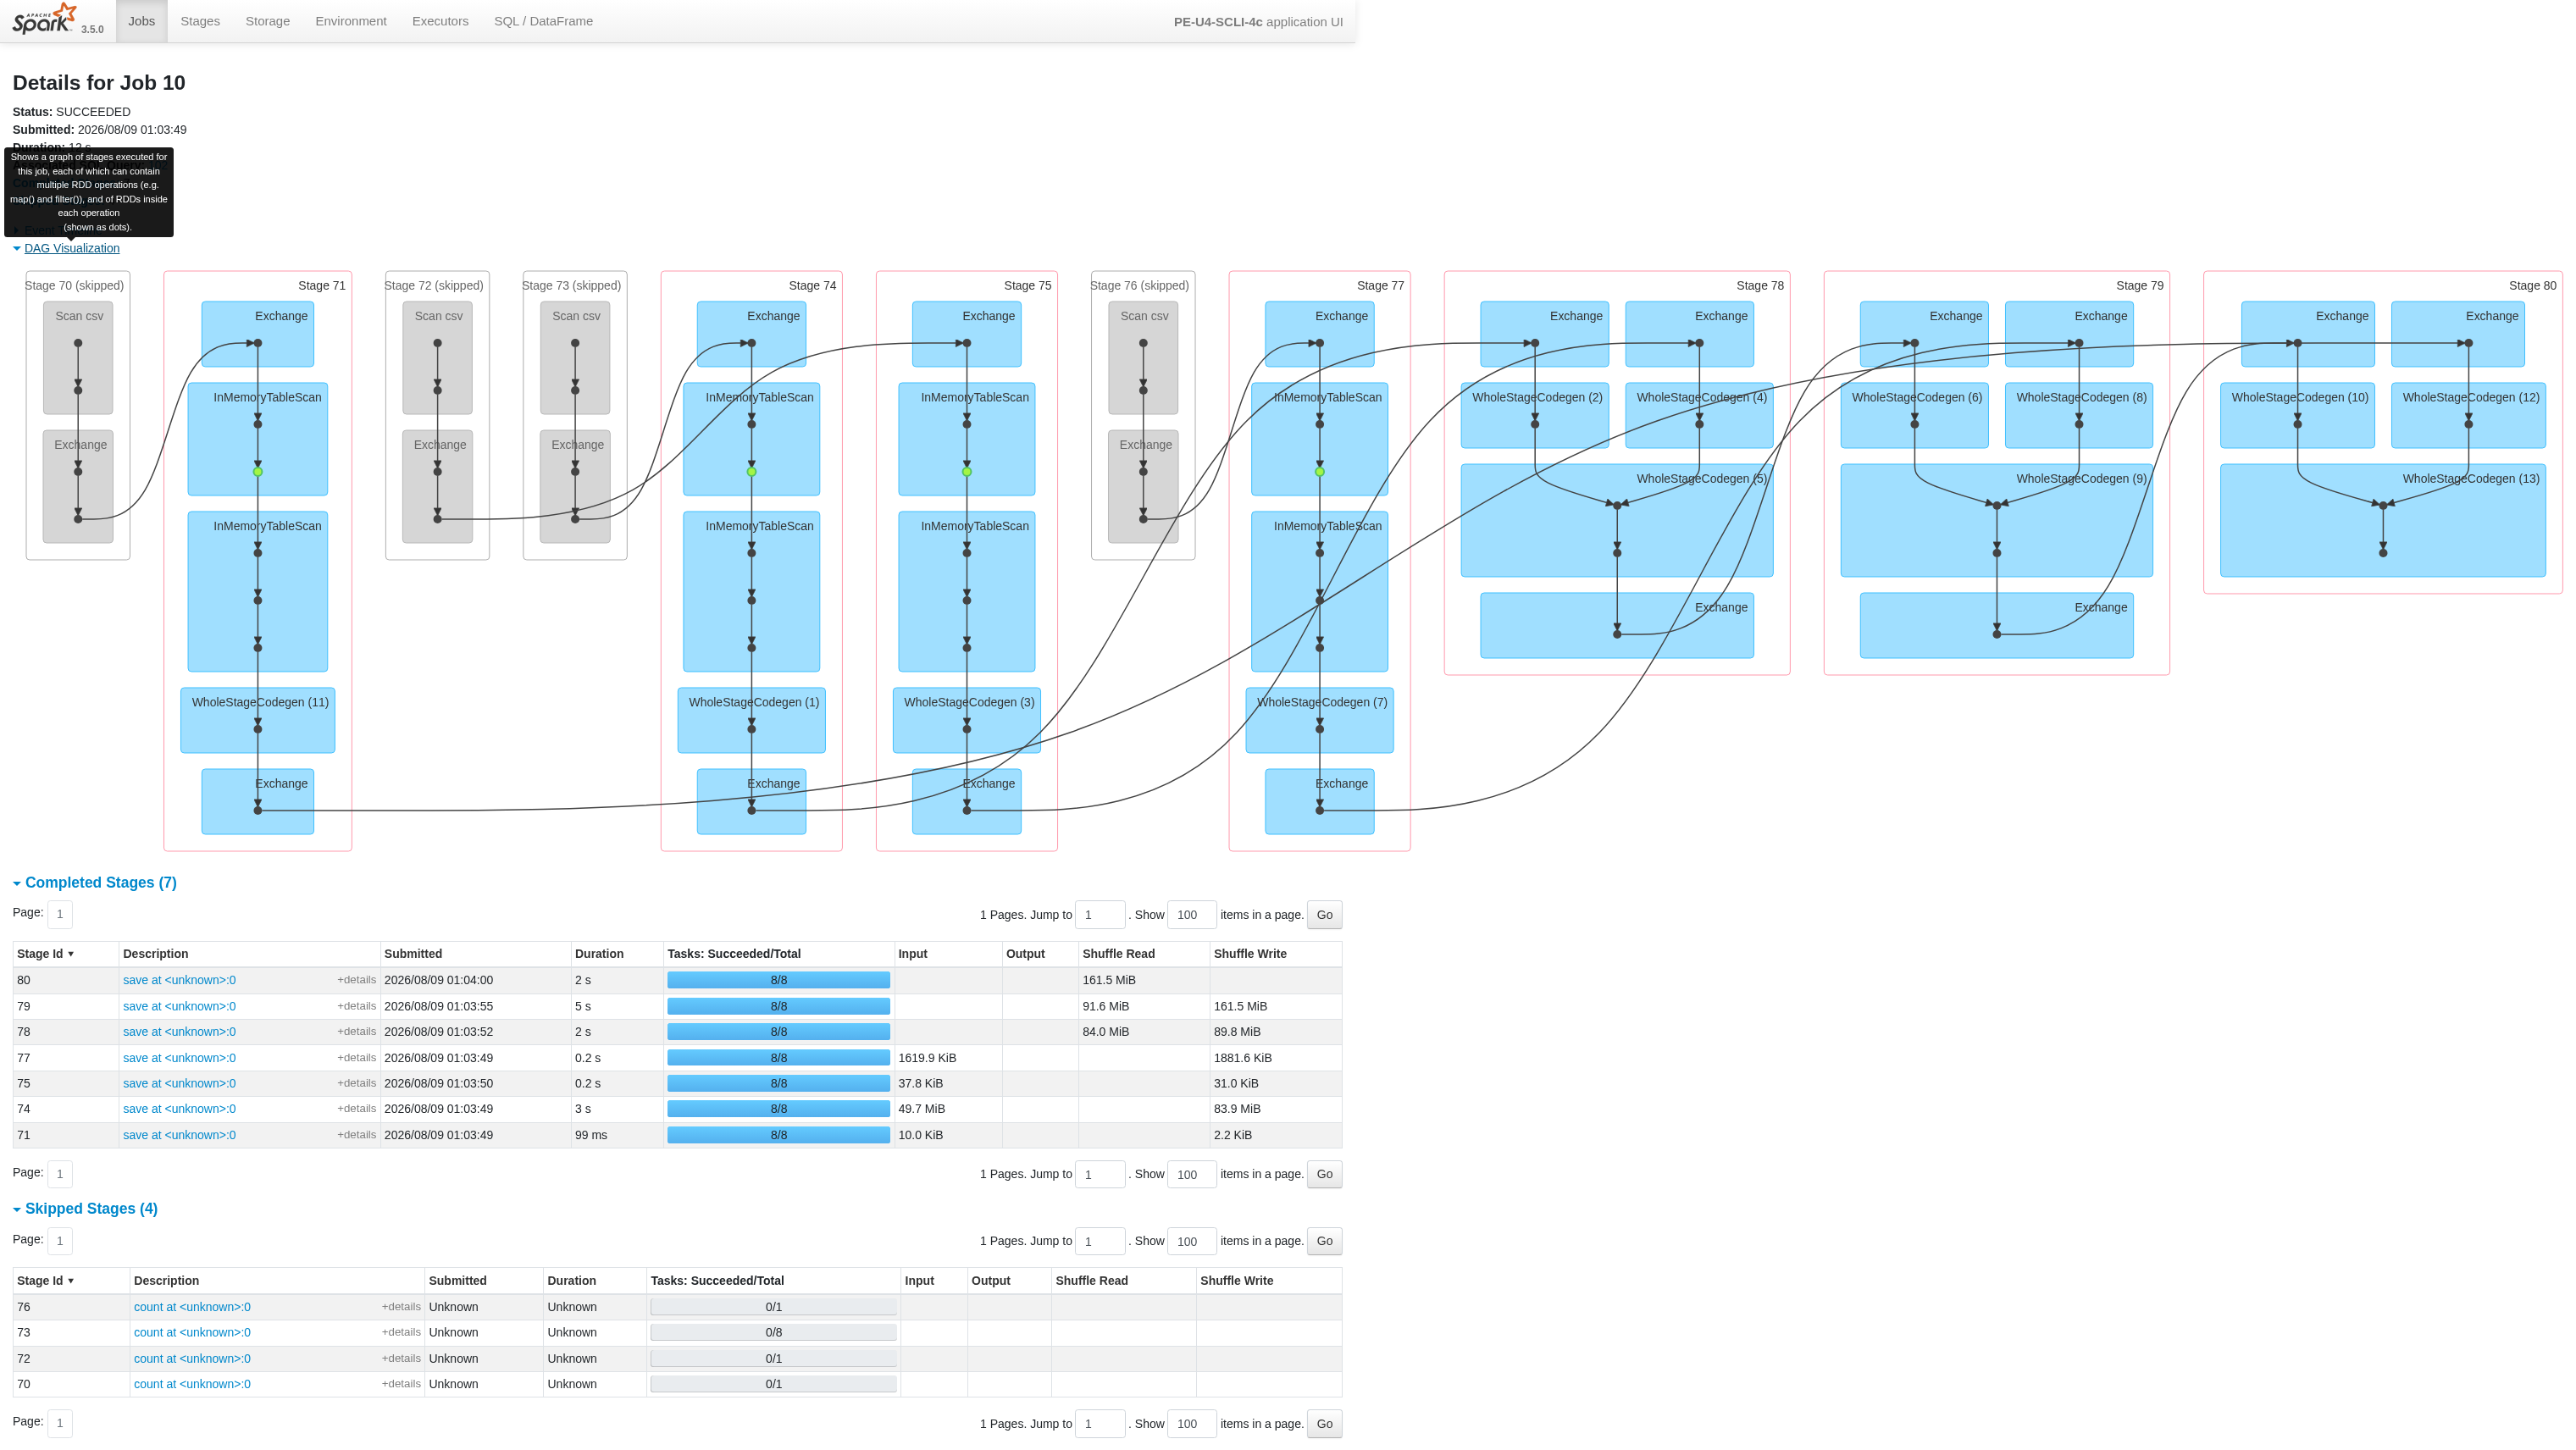
\includegraphics[width=.98\textwidth]{spark_ui_t3.png}
\caption{DAG y stages del job de T3 observados en Spark UI.}
\label{fig:spark-ui}
\end{figure}
La figura~\ref{fig:spark-ui} muestra el job completado, siete stages ejecutados y varios nodos \emph{Exchange}. Esos intercambios corresponden a fronteras de shuffle y respaldan la explicación de la sobrecarga de la unión distribuida.

\section{Análisis cuantitativo de Amdahl}
Para T3 se tomó como referencia el tiempo con una unidad, $T(1)=\SI{11.980450}{\second}$. Con dos unidades, $T(2)=\SI{11.880410}{\second}$, por lo que
\begin{equation}
S(2)=\frac{11.980450}{11.880410}=1.0084.
\label{eq:s2}
\end{equation}
Con cuatro unidades, $T(4)=\SI{9.909173}{\second}$:
\begin{equation}
S(4)=\frac{11.980450}{9.909173}=1.2090.
\label{eq:s4}
\end{equation}
La fracción no escalable observada se obtiene mediante Karp--Flatt:
\begin{equation}
e(N)=\frac{\frac{1}{S(N)}-\frac{1}{N}}{1-\frac{1}{N}},\qquad N>1.
\label{eq:karpflatt}
\end{equation}
Al sustituir $N=2$ y $S(2)=1.0084$, se obtiene $e(2)=0.9833$. Para $N=4$ y $S(4)=1.2090$, resulta $e(4)=0.7695$. Estos valores no representan únicamente código serial: agregan planificación, materialización, shuffle, serialización y competencia por CPU. La fracción paralelizable media estimada por el programa fue $p=0.1236$, por lo que
\begin{equation}
S_{\max}=\frac{1}{1-0.1236}=1.1410.
\label{eq:smax-numerico}
\end{equation}
El resultado debe interpretarse como una aproximación experimental sensible a la variabilidad. De hecho, $S(4)=1.2090$ supera el límite calculado con el promedio de solo dos estimaciones; esa discrepancia señala que la fracción observada no es constante y que el modelo ideal no incorpora las variaciones del entorno. Karbowski recuerda que las leyes clásicas omiten comunicación y sincronización, por lo que el speedup real queda condicionado por factores externos al reparto ideal \cite{karbowski2025}.

\section{Preguntas de análisis}
\subsection{Speedup máximo de T3 y 90\% del límite}
El cálculo experimental produjo $p=0.1236$ y, mediante la ecuación~\eqref{eq:smax-numerico}, un límite de 1,1410. El 90\% de ese valor es $0.9(1.1410)=1.0269$. Al resolver la ecuación de Amdahl para ese objetivo, el programa obtiene $N=1.27$, que se redondea a dos unidades. Sin embargo, el punto medido con $N=2$ fue 1,0084, ligeramente inferior al objetivo teórico. Esto demuestra que el número calculado no constituye una garantía de rendimiento, sino una predicción bajo la hipótesis de sobrecarga nula. Spark debe crear tareas, coordinar stages y mover datos entre particiones, costes que no aparecen en la ecuación ideal.

La medición con cuatro unidades alcanzó 1,2090, pero Colab solo reportó dos núcleos físicos. Por tanto, \texttt{local[4]} representa cuatro hilos que compiten sobre dos núcleos y no cuatro procesadores independientes. La variación entre repeticiones y el comportamiento del entorno compartido pueden explicar que ese punto supere el límite estimado a partir de una fracción promedio. La conclusión válida no es que se haya refutado Amdahl, sino que la estimación de $p$ resulta inestable con pocos puntos y con sobrecarga variable. Para fortalecer el resultado sería necesario repetir el barrido en una máquina con cuatro núcleos físicos dedicados y registrar más configuraciones. La relación entre Amdahl y Gustafson--Barsis también recuerda que la conclusión cambiaría si, en lugar de fijar 520,000 registros, el volumen creciera junto con los recursos \cite{karbowski2025}.

\subsection{Speedup menor que uno y umbral de rentabilidad}
El speedup pandas/Spark fue inferior a uno en todas las transformaciones. En T1, Spark tardó \SI{0.802504}{\second} frente a \SI{0.102893}{\second} de pandas; la diferencia fue \SI{0.699611}{\second}. En T3, la diferencia alcanzó \SI{9.767638}{\second}. Estas brechas incorporan planificación del DAG, creación de tareas, serialización, materialización y shuffle. Spark no acelera automáticamente una carga: la cantidad de trabajo paralelizable debe ser suficiente para amortizar esos costes.

La literatura sobre predicción de rendimiento destaca precisamente la interacción entre tamaño de entrada, configuración, capacidad del sistema y complejidad de la aplicación \cite{shen2023spark}. Con una única escala de 520,000 solicitudes no es posible calcular rigurosamente el volumen de cruce. Para estimarlo habría que medir, como mínimo, tres o cuatro tamaños de entrada, ajustar $T_{pandas}(n)=\alpha n$ y $T_{Spark}(n)=\beta+\gamma n/N$, y resolver $n^*=\beta/(\alpha-\gamma/N)$ cuando el denominador sea positivo. Por debajo de ese umbral, FUVV debería utilizar pandas o consultas SQL programadas; por encima, podría considerar Spark si el historial y las uniones crecen lo suficiente. La respuesta técnicamente honesta es que el experimento actual demuestra que 520,000 registros no justifican Spark en este entorno, pero no determina todavía un umbral numérico defendible. Inventarlo a partir de una sola escala contradiría la trazabilidad exigida.

\subsection{Integración mediante Structured Streaming}
\pendiente{Isaías}{Redactar al menos 200 palabras sobre fuentes, destinos, disparadores, checkpoint, watermark y garantías de entrega, vinculándolo con la arquitectura real de FUVV y citando sus propias fuentes.}

\subsection{Ventaja frente a MapReduce en procesamiento iterativo}
\pendiente{Andy}{Redactar al menos 200 palabras comparando Spark y MapReduce mediante linaje, evaluación perezosa, reutilización en memoria y materialización intermedia. Debe relacionar el argumento con el DAG de la figura~\ref{fig:spark-ui} y añadir sus propias fuentes.}

\section{Análisis crítico}
El experimento no demuestra que Spark sea inadecuado en general. Demuestra que, para 520,000 solicitudes, dos núcleos físicos y cinco transformaciones ejecutadas una vez, el coste del motor supera el trabajo útil. T3 contiene varios intercambios y alcanza una mediana de \SI{11.277967}{\second}, mientras pandas resuelve la unión en \SI{1.510329}{\second}. T4 presenta un coeficiente de variación de Spark de 37,95\%, señal de que el entorno compartido introduce ruido considerable. En consecuencia, no sería correcto extrapolar estos valores a un clúster dedicado.

La arquitectura también debe ajustarse al tipo de evento. Un enfoque serverless puede atender validaciones breves y activadores sin mantener infraestructura permanente, pero introduce arranques en frío y dificultades de estado \cite{wen2023serverless}. Spark resulta más apropiado para lotes históricos amplios o flujos que reutilizan estado y ejecutan agregaciones complejas. En FUVV, la solución razonable es híbrida: procesamiento transaccional y eventos pequeños con servicios ligeros; analítica histórica con SQL, pandas o Spark según el volumen medido. Esta postura evita adoptar un motor distribuido únicamente por tendencia tecnológica.

\pendiente{Andy e Isaías}{Añadir su análisis crítico propio sobre datos, configuración de Spark, limitaciones y decisiones arquitectónicas.}

\section{Conclusiones individuales}
\subsection*{José Alejandro Lozano Morales}
La principal conclusión es que la reproducibilidad cambia la interpretación del rendimiento. Al conservar semilla, repeticiones, medianas, configuración, resultados y Spark UI, fue posible comprobar que los cinco speedups frente a pandas quedaron por debajo de uno y que T3 produjo siete stages con varios intercambios. El resultado no debe ocultarse ni ajustarse para aproximarlo a la teoría: con 520,000 registros y dos núcleos, la sobrecarga de Spark domina la ejecución. La Ley de Amdahl sigue siendo útil como referencia, pero su aplicación requiere reconocer que la fracción no escalable observada incorpora costes del motor y variabilidad del entorno. También se comprobó que \texttt{local[4]} no equivale a cuatro executors distribuidos ni a cuatro núcleos físicos. Para AGLS -- TiendaTech, esta evidencia aconseja reservar Spark para análisis históricos de catálogos, compatibilidades y comportamiento de compra cuyo volumen supere un umbral medido; para cargas menores serían preferibles SQL o pandas. La decisión tecnológica debe basarse en el volumen, la complejidad y el coste operacional, no en la expectativa de que distribuir una tarea siempre la acelera.

\subsection*{Andy Paul Sánchez Pilaloa}
\pendiente{Andy}{Redactar personalmente su conclusión individual de al menos 150 palabras, vinculada con su evidencia y su rol.}

\subsection*{Isaías Abraham Urbina Romero}
\pendiente{Isaías}{Redactar personalmente su conclusión individual de al menos 150 palabras, vinculada con su evidencia y su rol.}

\section*{Declaración de uso de inteligencia artificial generativa}
José Alejandro Lozano Morales utilizó OpenAI Codex para revisar la estructura del repositorio, adaptar su parte del documento LaTeX, organizar los resultados experimentales y comprobar la correspondencia de sus cuatro referencias bibliográficas. Las cifras se tomaron de los archivos versionados de la corrida y fueron contrastadas con el código y las evidencias. La redacción y las conclusiones deberán ser revisadas por José antes de la entrega. Andy Sánchez e Isaías Urbina deben añadir personalmente cualquier uso de IA realizado en sus secciones.

\pendiente{Andy e Isaías}{Declarar herramienta, propósito y secciones asistidas, si utilizaron IA generativa.}

\printbibliography
\end{document}
